\documentclass[11pt,a4paper]{article}
\usepackage[utf8]{inputenc}
\usepackage[T1]{fontenc}
\usepackage[colorlinks, pagebackref=true]{hyperref}
\usepackage{mathtools, amsthm, amsfonts, amssymb}
\usepackage{tikz}
\usetikzlibrary{decorations.markings}
\usetikzlibrary{arrows.meta}
\usepackage{xcolor}

\begin{document}

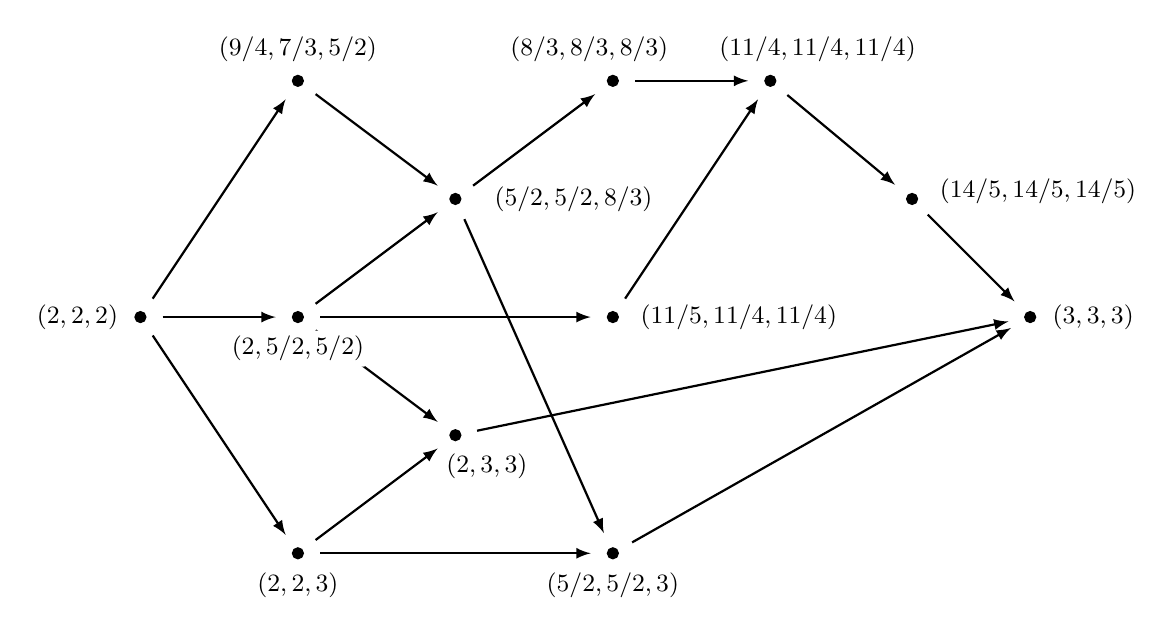
\begin{tikzpicture}
\def\s{1} %
\def\t{1} %

\coordinate (A) at (0*\s,0);
\coordinate (B) at (2*\s,-3*\t);
\coordinate (C) at (2*\s,0*\t);
\coordinate (D) at (2*\s,3*\t);

\coordinate (E) at (4*\s,-1.5*\t);
\coordinate (F) at (4*\s,1.5*\t);

\coordinate (G) at (6*\s,-3*\t);
\coordinate (H) at (6*\s,0*\t);
\coordinate (I) at (6*\s,3*\t);

\coordinate (J) at (8*\s,3*\t);
\coordinate (K) at (9.8*\s,1.5*\t);

\coordinate (L) at (11.3*\s,0*\t);


\draw[-latex, shorten >=8pt,shorten <=8pt, thick] (A) -- (B);
\draw[-latex, shorten >=8pt,shorten <=8pt, thick] (A) -- (C);
\draw[-latex, shorten >=8pt,shorten <=8pt, thick] (A) -- (D);
\draw[-latex, shorten >=8pt,shorten <=8pt, thick] (B) -- (E);
\draw[-latex, shorten >=8pt,shorten <=8pt, thick] (B) -- (G);
\draw[-latex, shorten >=8pt,shorten <=8pt, thick] (C) -- (E);
\draw[-latex, shorten >=8pt,shorten <=8pt, thick] (C) -- (H);
\draw[-latex, shorten >=8pt,shorten <=8pt, thick] (C) -- (F);
\draw[-latex, shorten >=8pt,shorten <=8pt, thick] (D) -- (F);
\draw[-latex, shorten >=8pt,shorten <=8pt, thick] (E) -- (L);
\draw[-latex, shorten >=8pt,shorten <=8pt, thick] (F) -- (G);
\draw[-latex, shorten >=8pt,shorten <=8pt, thick] (F) -- (I);
\draw[-latex, shorten >=8pt,shorten <=8pt, thick] (G) -- (L);
\draw[-latex, shorten >=8pt,shorten <=8pt, thick] (H) -- (J);
\draw[-latex, shorten >=8pt,shorten <=8pt, thick] (I) -- (J);
\draw[-latex, shorten >=8pt,shorten <=8pt, thick] (J) -- (K);
\draw[-latex, shorten >=8pt,shorten <=8pt, thick] (K) -- (L);


\draw[black, fill=black] (A) circle (2pt);
\draw (A) ++(-0.8,0) node {\small$(2,2,2)$};

\draw[black, fill=black] (B) circle (2pt);
\draw (B) ++(0,-0.4) node {\small$(2,2,3)$};

\draw[black, fill=black] (C) circle (2pt);
\draw (C) ++(0,-0.4) node[fill=white,rounded corners=2pt,inner sep=2pt] {\small$(2,5/2,5/2)$};

\draw[black, fill=black] (D) circle (2pt);
\draw (D) ++(0,0.4) node {\small$(9/4,7/3,5/2)$};

\draw[black, fill=black] (E) circle (2pt);
\draw (E) ++(0.4,-0.4) node[fill=white,rounded corners=2pt,inner sep=2pt]  {\small$(2,3,3)$};

\draw[black, fill=black] (F) circle (2pt);
\draw (F) ++(1.5, 0) node[fill=white,rounded corners=2pt,inner sep=2pt]   {\small$(5/2,5/2,8/3)$};

\draw[black, fill=black] (G) circle (2pt);
\draw (G) ++(0,-0.4) node[fill=white,rounded corners=2pt,inner sep=2pt] {\small$(5/2,5/2,3)$};

\draw[black, fill=black] (H) circle (2pt);
\draw (H) ++(1.6, 0) node {\small$(11/5,11/4,11/4)$};

\draw[black, fill=black] (I) circle (2pt);
\draw (I) ++(-0.3,0.4) node {\small$(8/3,8/3,8/3)$};

\draw[black, fill=black] (J) circle (2pt);
\draw (J) ++(0.6,0.4) node {\small$(11/4,11/4,11/4)$};

\draw[black, fill=black] (K) circle (2pt);
\draw (K) ++(1.6,0.1) node {\small$(14/5,14/5,14/5)$};

\draw[black, fill=black] (L) circle (2pt);
\draw (L) ++(0.8,0) node {\small$(3,3,3)$};

%
%
%

%
%
%
%
%
%

%
%
%
%
%

%
%
%

%
%
%

\end{tikzpicture}

\end{document}